\documentclass[12pt, tikz,border=6pt]{standalone}
\usetikzlibrary{arrows.meta,calc}

\begin{document}
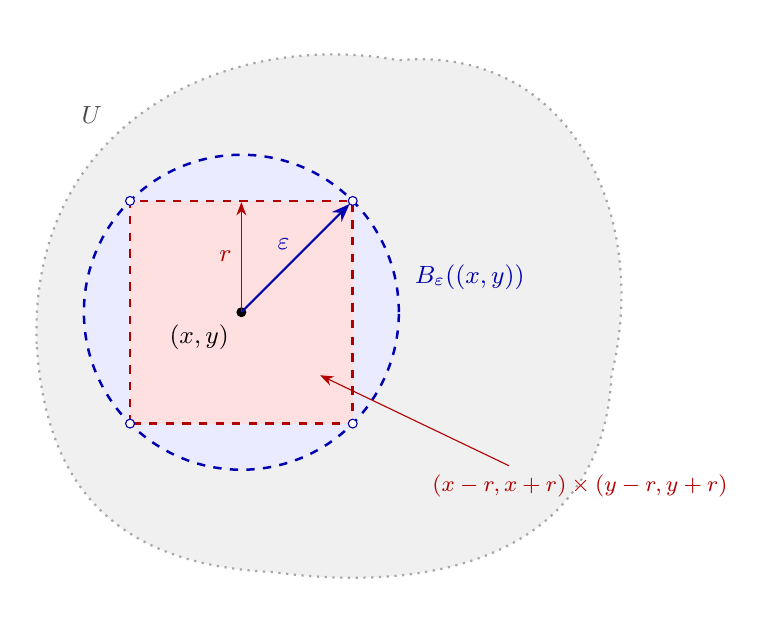
\begin{tikzpicture}[>=Stealth, every node/.style={font=\small}]
  \def\e{2}           % epsilon
  \pgfmathsetmacro{\r}{\e/sqrt(2)}

  % The open set U
\begin{scope}[shift={(1,0)}]
  \draw[fill=gray!12, draw=gray!70, dotted, line width=0.8pt]
    (-3.6,-0.4) .. controls (-3.7,2.4) and (-1.2,3.6) .. (1.0,3.2)
    .. controls (3.2,3.4) and (4.2,1.2) .. (3.7,-0.8)
    .. controls (3.6,-3.0) and (1.6,-3.6) .. (-0.6,-3.3)
    .. controls (-2.8,-3.2) and (-3.5,-2.0) .. (-3.6,-0.4) -- cycle;
  \node[gray!60!black] at (-2.9,2.5) {$U$};
\end{scope}

  % The open disk B_epsilon((x,y))
  \draw[fill=blue!8, draw=blue!70!black, line width=0.9pt, dashed] (0,0) circle (\e);

  % The open rectangle (square), dashed since it is open
  \draw[fill=red!12, draw=red!70!black, dashed, line width=0.9pt]
    (-\r,-\r) rectangle (\r,\r);

  % Corners lie on the boundary circle
  \foreach \sx/\sy in {1/1,1/-1,-1/1,-1/-1}
    \draw[fill=white, draw=blue!70!black] (\sx*\r,\sy*\r) circle (1.6pt);

  % Centre point
  \fill (0,0) circle (1.8pt) node[below left=1pt] {$(x,y)$};

  % Epsilon: radius to the corner
  \draw[->, blue!70!black, line width=0.8pt, shorten >= 1.6pt] (0,0) -- (\r,\r)
    node[midway, above left=-1pt] {$\varepsilon$};

  % r: half-side
  \draw[->, red!70!black, shorten >= 0.45pt] (0,0) -- (0,\r)
    node[midway, left] {$r$};

  % Labels
  \node[blue!70!black] at (2.9,0.45) {$B_\varepsilon((x,y))$};
  \node[red!70!black, align=center] at (4.3,-2.2) {\footnotesize$(x-r,x+r)\times(y-r,y+r)$};
  \draw[->, red!70!black] (3.4,-1.95) -- (1.0,-0.8);
\end{tikzpicture}
\end{document}
